\documentclass[a4paper]{article}% !TEX encoding = UTF-8 Unicode

\usepackage[T1]{fontenc}		% För svenska bokstäver
\usepackage[utf8]{inputenc}		% Teckenkodning UTF8
\usepackage[swedish]{babel}		% För svensk avstavning och svenska
                          		% rubriker (t ex "Innehållsförteckning")
\usepackage{hyperref} 			% Lägga till länkar i texten.
\usepackage{mathtools}			% Matematiska formler

\title{
	Krusty Kookies Sweden AB: Programmerings Projekt in Databasteknik (EDA216)\\
	EDA, Institutionen för Datavetenskap, Lunds Tekniska Högskola\\
	Per Holm}
\author{
Adam Hansson Lyrén, C11 (dic11aha@student.lu.se)\\
Mergim Rama, C11 (dic11mra@student.lu.se)\\
}


% *** Tillägg för denna rapport. ***
% Paket:
\usepackage{graphicx}         % För att inkludera bilder.

% Kommandon i denna rapport
\newcommand{\code}[1]{\texttt{#1}} % För programkod i text.
% *** Slut på tillägg för denna rapport. ***


\begin{document}              % Början på dokumentet

\maketitle
\centerline{
\includegraphics[scale = 0.6]{LTH.jpg}}
\thispagestyle{empty}

\newpage
\setcounter{page}{1}


\tableofcontents
\newpage

\section{Introduktion}

Projektets uppgift var att konstruera ett program som tar hand om alla delar som påverkas av en kakproduktion på företaget, allt från att tillverka en pall kakor, till att minska mängden råvaror på lagret. Vi ska även implementera funktioner för att blockera och söka på specifika pallar, vilka tillsammans presenteras i ett program som simulerar pallprodultionen. Allt detta kräver att man designat och implementerat en databas samt ett GUI för programmet.


\section{System}

Skriva om hur vi kopplar databasen till klasserna och vilka klasser det är som tar hand om kopplingen, vilka versioner av PHP MyQSL mm vi använder. Hur vi delat upp GUI klasserna. 



\section{Implementation}

Projektet består i grunden av två huvudsakliga implementationer, vilka är databasimplementationen samt GUI implementationen. Dessa implementationer har olika uppgifter i projektet. Databasen kommer stå för sparandet av viktig information samt att kunna få ut det man vi ha ut ur informationen. GUIt ska göra programmet användarvänligt så att även den minst tekniske ska kunna använda det utan att ha någon förkunskap om funktionaliteten.

\subsection{Databasimplementation}

Databasen vi implementerade är av typen MySQL och går att hitta på institutionens egna server som de tillhandager EDA216 studenter. Serverns adress är puccini.cs.lth.se. För att göra våra querys säkra mot attacker använder vi oss av preparedStatements, vilka vi skriver i php. 

Eftersom att flera ska vara inne samtidigt och utföra handlingar i databasen inte var ett krav så beslöt vi oss för att inte implementera transactions. All SQL kod vi använt för att skapa databasen går att hitta under \emph{6. Databasdump}.

\subsection{GUI Implementation}



Resultatet av hela projektet. Vad vi klarat av att implementera och vad vi inte gjort. Detta för att se hur mycket vi gjort. 

\section{Modellering}

Att få fram ett bra E/R diagram till programmet är inte lätt. Man måste läsa beskrivningen av problemet som introducerats och analysera det in i minsta detalj för att sedan kunna skapa ett skapligt diagram. Vi satte och och läste texten några gånger och fick slutligen fram en någorlunda design. Efter att ha filat och gjort om skickade vi in den till projektansvarige för att få bekräftelse på om diagrammet ser bra ut eller om det behöver någon ändring. 

När vi fick tillbaka feedbacken var det enstaka punkter som korrigerades. Nu kunde vi övergå till relationsöversättning för att sedan kunna implementera databasen. E/R diagrammet syns på bilden nedan. 

\subsection{E/R Diagram}
\centerline{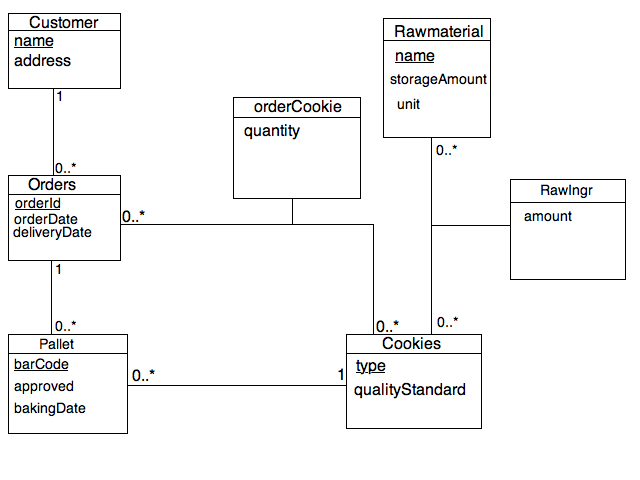
\includegraphics[scale = 0.6]{er.jpg}}

\section{Relationer}

Databasen vi har skapat består av 7 relationer varav två av relationerna är referenstabeller för många-till-många relationer. För att få fram en så korrekt databas som möjligt utgår man från det E/R diagram man modellerat och skapar relationerna utifrån den.

\subsection{Relationerna}
\begin{itemize}
	
\item{Customer(\underline{name}, address)}
\item{Order(\underline{orderId}, \emph{customerName}, orderDate, deliveryDate)}
\item{Cookies(\underline{type}, qStandard)}
\item{OrderCookie(\underline{\emph{orderId}}, \underline{\emph{cookieType}}, quantity)}
\item{Pallet(\underline{barCode}, \emph{cookieType}, \emph{orderId}, approved, bakingDate)}
\item{Rawmaterial(\underline{name}, storageAmount, unit)}
\item{Rawingr(\underline{\emph{cookieType}}, \underline{\emph{rawMaterialName}}, amount)}

\end{itemize}

Eftersom våra relationer saknar funktionella beroenden mellan attributen och att de endast har nyckelberoenden så är våra relationer i BCNF. 


\section{Databasdump}
CREATE TABLE `cookies` (
  `type` varchar(40) NOT NULL DEFAULT '',
  `qualityStandard` int(3) NOT NULL DEFAULT '90',
  PRIMARY KEY (`type`)
);

CREATE TABLE `rawingr` (
  `cookieType` varchar(40) NOT NULL DEFAULT '',
  `rawMaterialName` varchar(40) NOT NULL DEFAULT '',
  `amount` double(10,0) NOT NULL,
  PRIMARY KEY (`cookieType`,`rawMaterialName`),
   FOREIGN KEY (`cookieType`) REFERENCES `cookies` (`type`),
  FOREIGN KEY (`rawMaterialName`) REFERENCES `rawmaterial` (`name`)
);

CREATE TABLE `orders` (
  `orderId` int(10) NOT NULL AUTO_INCREMENT,
  `orderDate` date NOT NULL,
  `deliveryDate` date DEFAULT NULL,
  `customerName` varchar(40) NOT NULL DEFAULT '',
  PRIMARY KEY (`orderId`),
  FOREIGN KEY (`customerName`) REFERENCES `customer` (`name`)
);

CREATE TABLE `customer` (
  `name` varchar(40) NOT NULL DEFAULT '',
  `address` varchar(40) NOT NULL DEFAULT '',
  PRIMARY KEY (`name`)
);

CREATE TABLE `ordercookie` (
  `quantity` int(10) NOT NULL,
  `orderId` int(10) NOT NULL,
  `cookieType` varchar(40) NOT NULL,
  PRIMARY KEY (`orderId`,`cookieType`),
  FOREIGN KEY (`orderId`) REFERENCES `orders` (`orderId`),
  FOREIGN KEY (`cookieType`) REFERENCES `cookies` (`type`)
);

CREATE TABLE `rawmaterial` (
  `name` varchar(40) NOT NULL DEFAULT '',
  `storageAmount` double(10,0) NOT NULL,
  `unit` varchar(45) DEFAULT 'g',
  PRIMARY KEY (`name`)
);

CREATE TABLE `pallet` (
  `barCode` int(10) NOT NULL AUTO_INCREMENT,
  `cookieType` varchar(40) NOT NULL,
  `location` varchar(45) NOT NULL DEFAULT 'Freezing Storage',
  `orderId` int(10) NOT NULL,
  `approved` tinyint(4) NOT NULL DEFAULT '1',
  `bakingDate` date NOT NULL,
  PRIMARY KEY (`barCode`),
  FOREIGN KEY (`cookieType`) REFERENCES `cookies` (`type`),
  FOREIGN KEY (`orderId`) REFERENCES `orders` (`orderId`)
);



\end{document}
